%% bare_jrnl.tex
%% V1.4b
%% 2015/08/26
%% by Michael Shell
%% see http://www.michaelshell.org/
%% for current contact information.
%%
%% This is a skeleton file demonstrating the use of IEEEtran.cls
%% (requires IEEEtran.cls version 1.8b or later) with an IEEE
%% journal paper.
%%
%% Support sites:
%% http://www.michaelshell.org/tex/ieeetran/
%% http://www.ctan.org/pkg/ieeetran
%% and
%% http://www.ieee.org/

%%*************************************************************************
%% Legal Notice:
%% This code is offered as-is without any warranty either expressed or
%% implied; without even the implied warranty of MERCHANTABILITY or
%% FITNESS FOR A PARTICULAR PURPOSE! 
%% User assumes all risk.
%% In no event shall the IEEE or any contributor to this code be liable for
%% any damages or losses, including, but not limited to, incidental,
%% consequential, or any other damages, resulting from the use or misuse
%% of any information contained here.
%%
%% All comments are the opinions of their respective authors and are not
%% necessarily endorsed by the IEEE.
%%
%% This work is distributed under the LaTeX Project Public License (LPPL)
%% ( http://www.latex-project.org/ ) version 1.3, and may be freely used,
%% distributed and modified. A copy of the LPPL, version 1.3, is included
%% in the base LaTeX documentation of all distributions of LaTeX released
%% 2003/12/01 or later.
%% Retain all contribution notices and credits.
%% ** Modified files should be clearly indicated as such, including  **
%% ** renaming them and changing author support contact information. **
%%*************************************************************************


% *** Authors should verify (and, if needed, correct) their LaTeX system  ***
% *** with the testflow diagnostic prior to trusting their LaTeX platform ***
% *** with production work. The IEEE's font choices and paper sizes can   ***
% *** trigger bugs that do not appear when using other class files.       ***                          ***
% The testflow support page is at:
% http://www.michaelshell.org/tex/testflow/


\documentclass[journal]{IEEEtran}
%
% If IEEEtran.cls has not been installed into the LaTeX system files,
% manually specify the path to it like:
% \documentclass[journal]{../sty/IEEEtran}



% Some very useful LaTeX packages include:
% (uncomment the ones you want to load)


% *** MISC UTILITY PACKAGES ***
%
%\usepackage{ifpdf}
% Heiko Oberdiek's ifpdf.sty is very useful if you need conditional
% compilation based on whether the output is pdf or dvi.
% usage:
% \ifpdf
%   % pdf code
% \else
%   % dvi code
% \fi
% The latest version of ifpdf.sty can be obtained from:
% http://www.ctan.org/pkg/ifpdf
% Also, note that IEEEtran.cls V1.7 and later provides a builtin
% \ifCLASSINFOpdf conditional that works the same way.
% When switching from latex to pdflatex and vice-versa, the compiler may
% have to be run twice to clear warning/error messages.


% *** CITATION PACKAGES ***
%
\usepackage{cite}
% cite.sty was written by Donald Arseneau
% V1.6 and later of IEEEtran pre-defines the format of the cite.sty package
% \cite{} output to follow that of the IEEE. Loading the cite package will
% result in citation numbers being automatically sorted and properly
% "compressed/ranged". e.g., [1], [9], [2], [7], [5], [6] without using
% cite.sty will become [1], [2], [5]--[7], [9] using cite.sty. cite.sty's
% \cite will automatically add leading space, if needed. Use cite.sty's
% noadjust option (cite.sty V3.8 and later) if you want to turn this off
% such as if a citation ever needs to be enclosed in parenthesis.
% cite.sty is already installed on most LaTeX systems. Be sure and use
% version 5.0 (2009-03-20) and later if using hyperref.sty.
% The latest version can be obtained at:
% http://www.ctan.org/pkg/cite
% The documentation is contained in the cite.sty file itself.

% images
\usepackage{graphicx}




% *** GRAPHICS RELATED PACKAGES ***
%
\ifCLASSINFOpdf
  % \usepackage[pdftex]{graphicx}
  % declare the path(s) where your graphic files are
  % \graphicspath{{../pdf/}{../jpeg/}}
  % and their extensions so you won't have to specify these with
  % every instance of \includegraphics
  % \DeclareGraphicsExtensions{.pdf,.jpeg,.png}
\else
  % or other class option (dvipsone, dvipdf, if not using dvips). graphicx
  % will default to the driver specified in the system graphics.cfg if no
  % driver is specified.
  % \usepackage[dvips]{graphicx}
  % declare the path(s) where your graphic files are
  % \graphicspath{{../eps/}}
  % and their extensions so you won't have to specify these with
  % every instance of \includegraphics
  % \DeclareGraphicsExtensions{.eps}
\fi
% graphicx was written by David Carlisle and Sebastian Rahtz. It is
% required if you want graphics, photos, etc. graphicx.sty is already
% installed on most LaTeX systems. The latest version and documentation
% can be obtained at: 
% http://www.ctan.org/pkg/graphicx
% Another good source of documentation is "Using Imported Graphics in
% LaTeX2e" by Keith Reckdahl which can be found at:
% http://www.ctan.org/pkg/epslatex
%
% latex, and pdflatex in dvi mode, support graphics in encapsulated
% postscript (.eps) format. pdflatex in pdf mode supports graphics
% in .pdf, .jpeg, .png and .mps (metapost) formats. Users should ensure
% that all non-photo figures use a vector format (.eps, .pdf, .mps) and
% not a bitmapped formats (.jpeg, .png). The IEEE frowns on bitmapped formats
% which can result in "jaggedy"/blurry rendering of lines and letters as
% well as large increases in file sizes.
%
% You can find documentation about the pdfTeX application at:
% http://www.tug.org/applications/pdftex





% *** MATH PACKAGES ***
%
\usepackage{amsmath}
\usepackage{mathtools}
% A popular package from the American Mathematical Society that provides
% many useful and powerful commands for dealing with mathematics.
%
% Note that the amsmath package sets \interdisplaylinepenalty to 10000
% thus preventing page breaks from occurring within multiline equations. Use:
%\interdisplaylinepenalty=2500
% after loading amsmath to restore such page breaks as IEEEtran.cls normally
% does. amsmath.sty is already installed on most LaTeX systems. The latest
% version and documentation can be obtained at:
% http://www.ctan.org/pkg/amsmath





% *** SPECIALIZED LIST PACKAGES ***
%
%\usepackage{algorithmic}
% algorithmic.sty was written by Peter Williams and Rogerio Brito.
% This package provides an algorithmic environment fo describing algorithms.
% You can use the algorithmic environment in-text or within a figure
% environment to provide for a floating algorithm. Do NOT use the algorithm
% floating environment provided by algorithm.sty (by the same authors) or
% algorithm2e.sty (by Christophe Fiorio) as the IEEE does not use dedicated
% algorithm float types and packages that provide these will not provide
% correct IEEE style captions. The latest version and documentation of
% algorithmic.sty can be obtained at:
% http://www.ctan.org/pkg/algorithms
% Also of interest may be the (relatively newer and more customizable)
% algorithmicx.sty package by Szasz Janos:
% http://www.ctan.org/pkg/algorithmicx




% *** ALIGNMENT PACKAGES ***
%
%\usepackage{array}
% Frank Mittelbach's and David Carlisle's array.sty patches and improves
% the standard LaTeX2e array and tabular environments to provide better
% appearance and additional user controls. As the default LaTeX2e table
% generation code is lacking to the point of almost being broken with
% respect to the quality of the end results, all users are strongly
% advised to use an enhanced (at the very least that provided by array.sty)
% set of table tools. array.sty is already installed on most systems. The
% latest version and documentation can be obtained at:
% http://www.ctan.org/pkg/array


% IEEEtran contains the IEEEeqnarray family of commands that can be used to
% generate multiline equations as well as matrices, tables, etc., of high
% quality.


% *** SUBFIGURE PACKAGES ***
%\ifCLASSOPTIONcompsoc
%  \usepackage[caption=false,font=normalsize,labelfont=sf,textfont=sf]{subfig}
%\else
%  \usepackage[caption=false,font=footnotesize]{subfig}
%\fi
% subfig.sty, written by Steven Douglas Cochran, is the modern replacement
% for subfigure.sty, the latter of which is no longer maintained and is
% incompatible with some LaTeX packages including fixltx2e. However,
% subfig.sty requires and automatically loads Axel Sommerfeldt's caption.sty
% which will override IEEEtran.cls' handling of captions and this will result
% in non-IEEE style figure/table captions. To prevent this problem, be sure
% and invoke subfig.sty's "caption=false" package option (available since
% subfig.sty version 1.3, 2005/06/28) as this is will preserve IEEEtran.cls
% handling of captions.
% Note that the Computer Society format requires a larger sans serif font
% than the serif footnote size font used in traditional IEEE formatting
% and thus the need to invoke different subfig.sty package options depending
% on whether compsoc mode has been enabled.
%
% The latest version and documentation of subfig.sty can be obtained at:
% http://www.ctan.org/pkg/subfig




% *** FLOAT PACKAGES ***
%
%\usepackage{fixltx2e}
% fixltx2e, the successor to the earlier fix2col.sty, was written by
% Frank Mittelbach and David Carlisle. This package corrects a few problems
% in the LaTeX2e kernel, the most notable of which is that in current
% LaTeX2e releases, the ordering of single and double column floats is not
% guaranteed to be preserved. Thus, an unpatched LaTeX2e can allow a
% single column figure to be placed prior to an earlier double column
% figure.
% Be aware that LaTeX2e kernels dated 2015 and later have fixltx2e.sty's
% corrections already built into the system in which case a warning will
% be issued if an attempt is made to load fixltx2e.sty as it is no longer
% needed.
% The latest version and documentation can be found at:
% http://www.ctan.org/pkg/fixltx2e
\usepackage{booktabs,ragged2e}
\usepackage[flushleft]{threeparttable}
\renewcommand\TPTtagStyle{\textit}
\usepackage[strings]{underscore}

%\usepackage{stfloats}
% stfloats.sty was written by Sigitas Tolusis. This package gives LaTeX2e
% the ability to do double column floats at the bottom of the page as well
% as the top. (e.g., "\begin{figure*}[!b]" is not normally possible in
% LaTeX2e). It also provides a command:
%\fnbelowfloat
% to enable the placement of footnotes below bottom floats (the standard
% LaTeX2e kernel puts them above bottom floats). This is an invasive package
% which rewrites many portions of the LaTeX2e float routines. It may not work
% with other packages that modify the LaTeX2e float routines. The latest
% version and documentation can be obtained at:
% http://www.ctan.org/pkg/stfloats
% Do not use the stfloats baselinefloat ability as the IEEE does not allow
% \baselineskip to stretch. Authors submitting work to the IEEE should note
% that the IEEE rarely uses double column equations and that authors should try
% to avoid such use. Do not be tempted to use the cuted.sty or midfloat.sty
% packages (also by Sigitas Tolusis) as the IEEE does not format its papers in
% such ways.
% Do not attempt to use stfloats with fixltx2e as they are incompatible.
% Instead, use Morten Hogholm'a dblfloatfix which combines the features
% of both fixltx2e and stfloats:
%
% \usepackage{dblfloatfix}
% The latest version can be found at:
% http://www.ctan.org/pkg/dblfloatfix




%\ifCLASSOPTIONcaptionsoff
%  \usepackage[nomarkers]{endfloat}
% \let\MYoriglatexcaption\caption
% \renewcommand{\caption}[2][\relax]{\MYoriglatexcaption[#2]{#2}}
%\fi
% endfloat.sty was written by James Darrell McCauley, Jeff Goldberg and 
% Axel Sommerfeldt. This package may be useful when used in conjunction with 
% IEEEtran.cls'  captionsoff option. Some IEEE journals/societies require that
% submissions have lists of figures/tables at the end of the paper and that
% figures/tables without any captions are placed on a page by themselves at
% the end of the document. If needed, the draftcls IEEEtran class option or
% \CLASSINPUTbaselinestretch interface can be used to increase the line
% spacing as well. Be sure and use the nomarkers option of endfloat to
% prevent endfloat from "marking" where the figures would have been placed
% in the text. The two hack lines of code above are a slight modification of
% that suggested by in the endfloat docs (section 8.4.1) to ensure that
% the full captions always appear in the list of figures/tables - even if
% the user used the short optional argument of \caption[]{}.
% IEEE papers do not typically make use of \caption[]'s optional argument,
% so this should not be an issue. A similar trick can be used to disable
% captions of packages such as subfig.sty that lack options to turn off
% the subcaptions:
% For subfig.sty:
% \let\MYorigsubfloat\subfloat
% \renewcommand{\subfloat}[2][\relax]{\MYorigsubfloat[]{#2}}
% However, the above trick will not work if both optional arguments of
% the \subfloat command are used. Furthermore, there needs to be a
% description of each subfigure *somewhere* and endfloat does not add
% subfigure captions to its list of figures. Thus, the best approach is to
% avoid the use of subfigure captions (many IEEE journals avoid them anyway)
% and instead reference/explain all the subfigures within the main caption.
% The latest version of endfloat.sty and its documentation can obtained at:
% http://www.ctan.org/pkg/endfloat
%
% The IEEEtran \ifCLASSOPTIONcaptionsoff conditional can also be used
% later in the document, say, to conditionally put the References on a 
% page by themselves.




% *** PDF, URL AND HYPERLINK PACKAGES ***
%
%\usepackage{url}
% url.sty was written by Donald Arseneau. It provides better support for
% handling and breaking URLs. url.sty is already installed on most LaTeX
% systems. The latest version and documentation can be obtained at:
% http://www.ctan.org/pkg/url
% Basically, \url{my_url_here}.




% *** Do not adjust lengths that control margins, column widths, etc. ***
% *** Do not use packages that alter fonts (such as pslatex).         ***
% There should be no need to do such things with IEEEtran.cls V1.6 and later.
% (Unless specifically asked to do so by the journal or conference you plan
% to submit to, of course. )


% correct bad hyphenation here
\hyphenation{op-tical net-works semi-conduc-tor}
\usepackage[british]{babel}
\usepackage[hidelinks, unicode]{hyperref}
\begin{document}
%
% paper title
% Titles are generally capitalized except for words such as a, an, and, as,
% at, but, by, for, in, nor, of, on, or, the, to and up, which are usually
% not capitalized unless they are the first or last word of the title.
% Linebreaks \\ can be used within to get better formatting as desired.
% Do not put math or special symbols in the title.
\title{Knuckle Finger Print Based Biometric Recognition:\\A Survey}
%
%
% author names and IEEE memberships
% note positions of commas and nonbreaking spaces ( ~ ) LaTeX will not break
% a structure at a ~ so this keeps an author's name from being broken across
% two lines.
% use \thanks{} to gain access to the first footnote area
% a separate \thanks must be used for each paragraph as LaTeX2e's \thanks
% was not built to handle multiple paragraphs
%

\author{Samuele Bortolotti (229326), Department of Information Engineering and Computer Science, University of Trento\\
\href{mailto:samuele.bortolotti@studenti.unitn.it}{\texttt{samuele.bortolotti@studenti.unitn.it}} }% <-this % stops a space
%\thanks{This paper was recommended by Associate Professor Nicola Conci.
%S. Bortolotti is with the Department of Information Engineering and Computer Science, University of Trento, Trento 38123, Italy (samuele.bortolotti@studenti.unitn.it).}}
%\thanks{Samuele Bortolotti was with the Department
%of Electrical and Computer Engineering, Georgia Institute of Technology, Atlanta,
%GA, 30332 USA e-mail: (see http://www.michaelshell.org/contact.html).}% <-this % stops a space
%\thanks{J. Doe and J. Doe are with Anonymous University.}% <-this % stops a space
%\thanks{Manuscript received April 19, 2005; revised August 26, 2015.}}



% note the % following the last \IEEEmembership and also \thanks - 
% these prevent an unwanted space from occurring between the last author name
% and the end of the author line. i.e., if you had this:
% 
% \author{....lastname \thanks{...} \thanks{...} }
%                     ^------------^------------^----Do not want these spaces!
%
% a space would be appended to the last name and could cause every name on that
% line to be shifted left slightly. This is one of those "LaTeX things". For
% instance, "\textbf{A} \textbf{B}" will typeset as "A B" not "AB". To get
% "AB" then you have to do: "\textbf{A}\textbf{B}"
% \thanks is no different in this regard, so shield the last } of each \thanks
% that ends a line with a % and do not let a space in before the next \thanks.
% Spaces after \IEEEmembership other than the last one are OK (and needed) as
% you are supposed to have spaces between the names. For what it is worth,
% this is a minor point as most people would not even notice if the said evil
% space somehow managed to creep in.



% The paper headers
% \markboth{Journal of \LaTeX\ Class Files,~Vol.~14, No.~8, August~2015}%
% {Shell \MakeLowercase{\textit{\textit{et al.}}}: Bare Demo of IEEEtran.cls for IEEE Journals}
% The only time the second header will appear is for the odd numbered pages
% after the title page when using the twoside option.
% 
% *** Note that you probably will NOT want to include the author's ***
% *** name in the headers of peer review papers.                   ***
% You can use \ifCLASSOPTIONpeerreview for conditional compilation here if
% you desire.




% If you want to put a publisher's ID mark on the page you can do it like
% this:
%\IEEEpubid{0000--0000/00\$00.00~\copyright~2015 IEEE}
% Remember, if you use this you must call \IEEEpubidadjcol in the second
% column for its text to clear the IEEEpubid mark.



% use for special paper notices
%\IEEEspecialpapernotice{(Invited Paper)}

% make the title area
\maketitle

% As a general rule, do not put math, special symbols or citations
% in the abstract or keywords.
\begin{abstract}
The automatic use of physiological or behavioral characteristics to determine or verify people identity is an arduous problem in computer vision which has been widely explored by researchers.
Human identification has been delved mainly through physiological biometrics, such as finger prints, iris, face and palm prints, and behavioral biometrics, such as voice and gaits. Biometrics combines image acquisition, feature extraction, signal processing and recognition systems and its application scenarios range from logical or physical access control to surveillance and law enforcement.
In terms of physical characteristics, the knuckle finger print comprises several different stable peculiar features which have made this surface relevant as a biometric identifier.
This paper reviews some of the literature on knuckle finger prints, discusses the methods for their acquisition and illustrates how to develop real-time human identification systems.
\end{abstract}

% Note that keywords are not normally used for perreview papers.
\begin{IEEEkeywords}
Biometrics, knuckle finger print, acquisition systems, recognition systems
\end{IEEEkeywords}





% For peer review papers, you can put extra information on the cover
% page as needed:
% \ifCLASSOPTIONpeerreview
% \begin{center} \bfseries EDICS Category: 3-BBND \end{center}
% \fi
%
% For peerreview papers, this IEEEtran command inserts a page break and
% creates the second title. It will be ignored for other modes.
\IEEEpeerreviewmaketitle



\section{Introduction}
% The very first letter is a 2 line initial drop letter followed
% by the rest of the first word in caps.
% 
% form to use if the first word consists of a single letter:
% \IEEEPARstart{A}{demo} file is ....
% 
% form to use if you need the single drop letter followed by
% normal text (unknown if ever used by the IEEE):
% \IEEEPARstart{A}{}demo file is ....
% 
% Some journals put the first two words in caps:
% \IEEEPARstart{T}{his demo} file is ....
% 
% Here we have the typical use of a "T" for an initial drop letter
% and "HIS" in caps to complete the first word.
%\IEEEPARstart{T}{his} demo file is intended to serve as a ``starter file''
%for IEEE journal papers produced under \LaTeX\ using
%IEEEtran.cls version 1.8b and later.
% You must have at least 2 lines in the paragraph with the drop letter
% (should never be an issue)
%I wish you the best of success.

\IEEEPARstart{T}{he} need for reliable user authentication techniques has significantly increased in the wake of heightened concerns about security and authentication~\cite{cryptography2010001}.

Biometric feature-based person identification methods find wider application than the conventional algorithms like knowledge based techniques, such as password based methods, PIN based methods and token based methods~\cite{Meraoumia}~\cite{DZhang} since they cannot be lost, transferred or stolen.

In computer science, biometrics is described as the automated recognition of people based on their physiological or behavioral features~\cite{Unar} which, according to Anil K. Jain \textit{et al.}~\cite{Jain}, can qualify as biometric traits if they comply with the following criteria: (i) universality, (ii) uniqueness, (iii) invariance, (iv) collectability, (v) performance, (vi) acceptability and (vii) circumvention.
Indeed, a biometric trait has to be universal, namely possessed by each individual, but at the same time unique since it must be sufficiently different among numerous human beings. Furthermore, it must not change over time (invariance) and it must be statistically quantified (collectability). As for its feasibility, a biometric identification system must be precise and quick in its recognition process (performance), as well as strong enough to avoid being easily manipulated through deception (circumvention)~\cite{Jain}.

This study focuses on \emph{Knuckle Finger Print} (KFP) which complies with Anil K. Jain \textit{et al.} definition.

According to recent studies~\cite{Meraoumia}~\cite{KumarKnuckle}~\cite{LiWenwen}, KFP constitutes a unique but efficient biometric trait, since it is rich in lines and creases which are reasonably stable over time and particularly distinctive among people.
The user acceptability of outer finger surface imaging is high, and data collection is straightforward and affordable.
Finally, human hand-based biometric information is particularly trustworthy. Hence, it may be used to accurately identify humans across a wide variety of demographics.

This paper presents a brief overview of KFP as a biometric descriptor. In particular~\hyperref[sec:acquisitionsystems]{Section II} discusses a possible acquisition method, ~\hyperref[sec:recognitionalgorithms]{Section III} provides some of the person's identification methods and a few datasets. Finally, ~\hyperref[sec:conclusion]{Section IV} presents the concluding remarks.

\section{Acquisition systems}
\label{sec:acquisitionsystems}
The act of sampling signals, which measure real-world physical conditions, and transforming the samples into digital numeric values is known as data acquisition. This process is possible by the means of sensors, signal conditioning circuitries and analog-to-digital converters.

Due to the lack of available datasets in the early stages of KFP recognition literature, the authors of several studies have built and explained data collection systems which are employed for both data collection and recognition~\cite{Zhang1}~\cite{Kumar}.

\begin{figure}
    \centering
    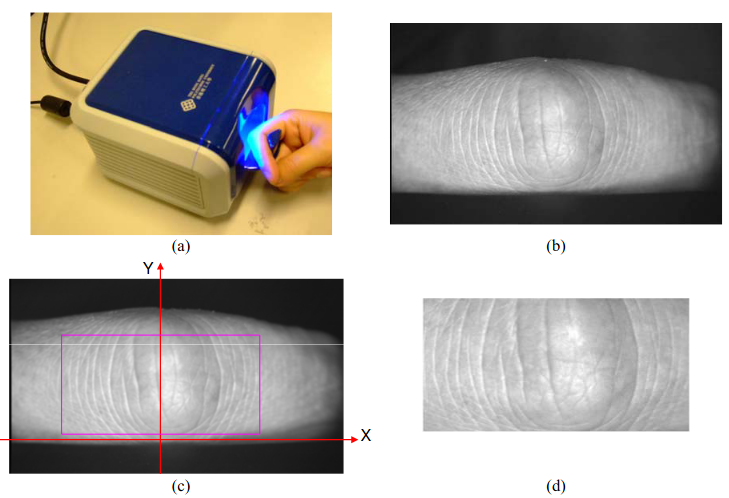
\includegraphics[width=2.5in]{images/zhang_acquisition_system.png}
    \caption{\textbf{(a)} KFP image acquisition device; \textbf{(b)} a KFP image; \textbf{(c)} ROI extraction; \textbf{(d)} cropped ROI image in (c). Courtesy of Lin Zhang \textit{et al.}}
    \label{fig:zhang_acq_sys}
\end{figure}

Lin Zhang \textit{et al.}~\cite{Zhang1} have provided a contactless 2D KFP biometric identifier for personal identity identification as an effective representation of a KFP acquisition mechanism. The proposed KFP image acquisition device, shown in Figure~\ref{fig:zhang_acq_sys}, is composed of a finger bracket, a ring LED light source, a lens, a CCD camera and a frame grabber. The data processing module receives the acquired KFP picture and performs three fundamental steps: \emph{Region Of Interest} (ROI) extraction, feature extraction and feature matching.

The ROI is identified through a 2D coordinate system. To begin with, the finger boundaries are determined by a Canny edge detector. The X-axis is then localized by fitting the finger border as a straight line, whereas the Y-axis is determined by the phalanges' orientation. Finally, the ROI is cropped for the feature extraction~\cite{LiWenwen}.

\section{Recognition algorithms}
\label{sec:recognitionalgorithms}
In the literature, a KFP recognition algorithm is generally described though two stages: a feature extraction algorithm and a matching algorithm, either based on distances or scores or classifiers.

The performance of a biometric system is typically quantified though a \emph{Receiver Operating Characteristic} (ROC) curve~\cite{Zhang1}\cite{ZHANG20111990}. To evaluate the results, two types of error rates are defined: \emph{False Acceptance Rate} (FAR), namely the probability that the system incorrectly authorizes a non-authorized person, and \emph{False Rejection Rate} (FRR), which is the probability that the system incorrectly rejects access to an authorized person. 
As a performance measure, the biometric system employs either the \emph{Recognition Rate} (RR) or the \emph{Equal Error Rate} (EER).
The RR measures the accuracy of the biometric system, whereas EER is a metric which combines both FRR and FAR, \textit{i.e.} the point in the ROC curve where the FAR is equal to the FRR. 
A system is considered highly accurate when the EER is low and the RR is high. 

With the outbreak and the development of neural networks, the techniques in the biometric recognition field have drastically changed. Therefore, it is possible to distinguish two phases in the literature, which correspond approximately to the period before 2012 and the one after 2012. In the first stage, the approaches were mostly based on traditional techniques such as filters, transforms and texture-based methods, whereas, due to recent advances, the newly proposed systems are based on deep neural networks.

This paper provides a classification of recognition algorithms similar to the one proposed by David Zhang \textit{et al.}~\cite{classification}, which comprises three categories: holistic-based, feature-based and hybrid methods.
In addition, this survey presents a brief discussion about the most recent deep neural networks approaches. Finally, the last part of this section describes concisely the available KFP datasets.

\subsection{Holistic-based methods}
In the holistic-based recognition approach, the KFP image is wholly used as input of a feature extractor, whose output is subsequently given to a matching algorithm~\cite{biometricknuckleprint} to complete the recognition procedure. Most holistic-based approaches in the literature employ subspace techniques and spectral representation.

\subsubsection{Subspace methods}
Subspace methods are characterized by the detection of spatially localized features in the image~\cite{KumarKnuckle}. The majority of subspace approaches in the literature are based on unsupervised subspace learning, which reduces data dimensionality while keeping the original data structure~\cite{Jing}. Some of the main techniques are \emph{Principal Component Analysis} (PCA), \emph{Independent Component Analysis} (ICA) and \emph{Linear Discriminate Analysis} (LDA). % anche qua citare

As an effective representation, Yang \textit{et al.}~\cite{WankouYANG:374} have proposed a KFP recognition method based on Gabor filters, PCA and \emph{Orthogonal Linear Discriminant
Analysis} (OLDA).

Gabor filters are band-pass filters with different frequencies and orientations. In the literature, those filters have been used to localize and extract local features of the KFP, namely magnitude, phase, and orientation\cite{ZHANG20111990} (see Figure~\ref{fig:gabor_filter}).

\begin{figure}
    \centering
    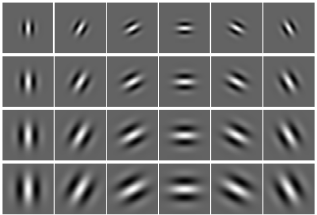
\includegraphics[width=2.0in]{images/gabor_filter.png}
    \caption{Bank of the 24 2D Gabor filters with four scales and six orientations. Courtesy of Lin Zhang \textit{et al.}}
    \label{fig:gabor_filter}
\end{figure}

Yang \textit{et al.} have initially constructed an enhanced Gabor feature vector which included all the elements acquired from the Gabor filter. However, since the Gabor feature representation is located in a very high-dimensional space, PCA is used to generate a meaningful low-dimensional representation in order to increase pattern matching computational efficiency and conserve space.
Yang \textit{et al.} have employed a LDA extension called OLDA with the aim of learning the subspace on which the classification is performed. The major issue of the standard LDA is that its formulation demands non-singular scatter matrices. However, when the data dimension is substantially bigger than the sample size, all scatter matrices are singular, thus LDA inevitably fails~\cite{nullspace}. 
Due to the orthogonalization provided by its constraints, OLDA solves the singularity problem.
Immediately after the feature extraction, a nearest neighbor classifier based on cosine distance is employed to perform the prediction.
Yang \textit{et al.} have evaluated the proposed technique on the Poly-U database~\cite{polyu1} achieving a maximum RR of 98.67\% and a minimum RR of 90\%.

\subsubsection{Spectral representation}
In spectral representation-based approaches the picture is converted from the spatial domain to another domain (Fourier, Gabor, \textit{etc.}), either to improve the image quality, or to extract the features' coefficients which will be employed in the recognition process~\cite{biometricknuckleprint}.

Meraoumia \textit{et al.}~\cite{Meraoumia} have suggested a robust spectral representation-based recognition system developed on the Fourier transform which considers two modalities: KFP and palm print.
To perform the recognition, Meraoumia \textit{et al.} have used the \emph{Phase-Correlation Function} (PCF), a well-known picture alignment approach. When two images are comparable, PCF produces a sharp peak, dramatically declining when they are not similar.
As a result, the height of the PCF peak has been employed as the similarity metric for matching the 2D discrete Fourier transform of the KFP and palm print pictures.
During the first stage, KFP and palm print pictures have been compared to those already stored in the database.
When the two unimodal biometric matching scores are computed, they are fused together employing a score level fusion based on the sum rule. Score level fusion refers to the combination of various matching scores provided by the unimodal classifiers. However, before proceeding to the fusion stage, the matching scores must be normalized; to accomplish this, Meraoumia \textit{et al.} have used the Min-Max method.

Assume the score vector is $D_i = [D_{i0}, D_{i1}, D_{i2}, \dots D_{iN}]$, where $N$ depicts the size of the system database and $i$ indicates the picture on which the method is being tested.
The normalized scores are calculated as follows: 
\begin{align*}
    DN_i = \frac{D_i - \min(D_i)}{\max(D_i) - \min(D_i)} \label{eq:2}
\end{align*}
where $DN_i$ is the normalized vector. The final decision is made according to the score obtained from the sum rule: for instance, if $D_0$ and $D_1$ represent the normalized scores associated to the FKP and to the palm print modalities, then the final score, $SF$, is defined as the sum between $D_0$ and $D_1$.

Meraoumia \textit{et al.} have evaluated the suggested technique on the Poly-U KFP database~\cite{polyu1} in combination with the palm print database, which is provided by the same university, achieving a RR of 97.417\% and an EER of 5.688\%.

\subsection{Feature-based}
Feature-based methods consist in the extraction of local prominent characteristics (such as edges, lines, \textit{etc.}) from the KFP images, and in the comparison with the stored templates by the means of a matching algorithm. 
In the literature, the feature-based approaches are mostly either coding-based or texture-based.

\subsubsection{Coding-based methods}
Coding-based systems use binary coding to encode the representation of KFP pictures. These techniques are frequently implemented using Wavelets or Gabor filters~\cite{biometricknuckleprint}.

In order to extract the local features of the KFP, Lin Zhang \textit{et al.}~\cite{Zhang1} have applied a simple and cost-effective coding method based on Gabor filters (see Figure~\ref{fig:gabor_filter}). The orientation information retrieved by the Gabor filter is then coded using a competitive coding scheme, referred as CompCode~\cite{ZHANG20111990}. CompCode involves the convolution operation between the points of the pre-processed image and the real part of the Gabor filter allowing to retrieve robust and brightness-independent features.
To determine whether two KFP images refer to the same finger, Lin Zhang \textit{et al.} have employed a matching algorithm on top of the extracted competitive code maps using the angular distance, namely a normalized hamming distance between the competitive codes. As a result, the final matching distance is the minimum of the resulting distances.

The verification phase has been performed on their proprietary database; through their experiments, Lin Zhang \textit{et al.} have achieved an EER of 1.09\% and a RR of 97.96%.

\subsubsection{Texture-based methods}
Texture-based approaches are feature-based methods which extract useful picture descriptors based on the image typical patterns.

Morales \textit{et al.}~\cite{morales2011improved} have suggested a method for FKP authentication based on Gabor filters and on the \emph{Scale Invariant Feature Transform} (SIFT) algorithm as an effective representation.

SIFT is a prominent texture identification approach which is invariant to picture scaling, rotation, and partial changes in illumination. 

Firstly, SIFT applies a Gaussian low-pass filter to the Gabor-processed KFP picture, which is then equalized using a histogram equalization technique (CLAHE). Secondly, the image keypoints are extracted (see Figure~\ref{fig:sift_descriptors}). Finally, the keypoints are used to extract the orientations and gradient magnitudes, namely the image descriptors. The Euclidean distance between keypoint descriptors is used as a similarity metric during the matching phase.

In summary, the analyzed KFP picture is linked to the closest match individual.
\begin{figure}
    \centering
    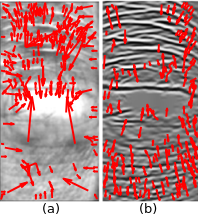
\includegraphics[width=1in]{images/sift.png}
    \caption{\textbf{(a)} SIFT over a FKP grayscale image; \textbf{(b)} SIFT over the pre-processed FKP grayscale image. Courtesy of Morales \textit{et al.}}
    \label{fig:sift_descriptors}
\end{figure}

Morales \textit{et al.} have tested the proposed approach on the Poly-U database~\cite{polyu1} obtaining an EER of 0.43\%.

\subsection{Hybrid methods}
Hybrid methods consists in the application of both holistic and local features in order to improve the recognition accuracy and enhance the identification speed.

As an effective representation, Lin Zhang \textit{et al.}~\cite{ZHANG20111990} have provided an extension of their previous work, enriching their coding method based on competitive coding scheme~\cite{Zhang1} with global features provided by the Fourier transform coefficients. The recognition process is performed by combining two distances. The first one is the angular distance based on the normalized hamming distance for the local orientation features. The second one is obtained with the \emph{Band-Limited Phase-Only Correlation} (BLPOC), a variation of the \emph{Phase-Only Correlation} (POC). Such distance measures the similarity of the two Fourier transforms obtained from the ROI of both of the KFP images. The BLPOC aims to estimate the relative translative offset between two similar images in the Fourier domain, avoiding noisy high frequency components. Once the local and global distances have been obtained, they are fused together by the means of a matcher-weighting rule distance; the resulting distance is subsequently used in the matching phase. Moreover, BLPOC is employed at the beginning of the process in order to align the KFP of the two evaluated pictures according to the location of the peak.

Lin Zhang \textit{et al.} have performed the verification phase on their own proprietary dataset achieving an EER of 0.402\% a FRR of 1.5236\% and a FAR of 0.0515\%.

\subsection{Deep neural networks methods}
Due to recent advances in Artificial Intelligence, deep neural networks have increasingly aroused interest in biometric identification. In the literature, those methods are mainly based on a \emph{Convolutional Neural Network} (CNN), a deep neural network architecture characterized by the combination of convolution and pooling layers.

A CNN is used either for feature extraction or classification; those tasks are commonly accomplished with the employment of a pre-trained model (\textit{e.g.} VGG or ResNet) trained on a big dataset such as ImageNet.

Tarawneh \textit{et al.}~\cite{tarawneh2022deepknuckle} have developed a KFP recognition pipeline based on the features extracted from the first two fully connected layers of VGG-19.
Following the features extraction, PCA is used to decrease the data dimensionality, preserving 95 percent of data variance. As a classifier, an \emph{Artificial Neural Network} (ANN), specifically a multilayer perceptron, has been trained and subsequently tested employing 5-fold-cross-validation.
The suggested technique outperforms well-known architectures such as Resnet18, while the state-of-the-art EfficientNet performs marginally better.

Tarawneh \textit{et al.} have performed the verification phase on the IIT Delhi Finger Knuckle Database~\cite{delhi} achieving an EER of 0.23\%.

\subsection{Datasets}
In order to test the performances of KFP recognition systems, several datasets have been introduced. In this section, the paper aims to provide a brief overview of the most relevant ones in the field of KFP.

\subsubsection{\texorpdfstring{Poly-U Finger-Knuckle Database~\cite{polyu1}}{Poly-U Finger-Knuckle Database}}
Provided by the Hong Kong Polytechnic University, the Poly-U Finger-Knuckle Database is one of the first KFP dataset to test human recognition algorithms. Altogether, the database contains 7,920 images from 660 different fingers obtained by 165 different individuals aged between 20 and 30 years old. The database contains KFP of the same finger acquired in two different sessions 4 to 7 years apart.

\subsubsection{\texorpdfstring{Lin Zhang \textit{et al.} dataset~\cite{ZHANG20111990}}{Lin Zhang \textit{et al.} dataset}}
Lin Zhang \textit{et al.} have established their own proprietary KFP dataset in order to evaluate their proposed KFP recognition techniques. The database contains 5,760 images from 480 different fingers obtained by 120 different individuals, aged between 30 and 50 years old. The dataset contains KFP of the same finger acquired in two different sessions 14 to 76 days apart.

\subsubsection{\texorpdfstring{IIT Delhi Finger Knuckle Database~\cite{delhi}}{IIT Delhi Finger Knuckle Database}}
The IIT Delhi established a KFP dataset including 790 images obtained by 158 different individuals aged between 16 and 55 years old.

\section{Conclusion}
\label{sec:conclusion}
This survey presented a brief description of the KFP-based biometric recognition, its definitions, a potential acquisition mechanism and an overview of some popular KFP datasets.

The purpose was to provide a general introduction of how a KFP recognition system works by discussing the major steps, from acquisition to image classification, as well as the main idea behind the various methodologies which may be used to fulfill the KFP recognition task.

As for the methods accuracy, all the presented KFP recognition algorithm categories have achieved astonishing results regardless of the methodologies employed, as illustrated in Table~\ref{tab:comparison}.

\begin{table}
\begin{threeparttable}
\caption{Accuracy Comparison of Different Recognition Methods based on KFP}
\label{tab:comparison}
\setlength\tabcolsep{0pt}

\begin{tabular*}{\columnwidth}{@{\extracolsep{\fill}} ll cccc}
\toprule
    Authors & Method\tnote{a} & Techniques\tnote{b} & Dataset &  \multicolumn{2}{c}{Accuracy (\%)}\tnote{c} \\ 
\cmidrule{5-6}
    & & & & EER & RR \\
\midrule
    Yang & Subspace & GF+OLDA & Poly-U & - & 98.67 \\
    Meraoumia & Spectral & 2D-DFT & Poly-U & 5.688 & 97.417 \\
\addlinespace
    Lin Zhang & Coding & GF+CC & Lin Zhang & 1.09 & 97.96 \\
    Morales & Texture & GF+SIFT & Poly-U & 0.43 & - \\
\addlinespace
    Lin Zhang & Hybrid & CC+BLPOC & Lin Zhang & 0.402 & - \\
\addlinespace
    Tarawneh & DNN & VGG-19+ANN & IIT Delhi & 0.23 & - \\
\bottomrule
\end{tabular*}

\smallskip
\scriptsize
\begin{tablenotes}
\RaggedRight
\item[a] DNN: Deep Neural Network

\item[b] GF: Gabor Filters; 
         DTF: Discrete Fourier Transform; 
         CC: Competitive Code;
         SIFT: Scale Invariant Feature Transform;
         BLPOC: Band-Limited Phase-Only Correlation;
         ANN: Artificial Neural Network

\item[c] -: Not Recorded;
         RR: Recognition Rate; 
         EER: Equal Error Rate; 
\end{tablenotes}
\end{threeparttable}
\end{table}

Despite their simplicity, holistic-based techniques have shown great results, namely RRs of 98.67\% and 97.417\%.
Moreover, features retrieved by subspace-based approaches are stable to changes such as illumination and position variation, however, the data has high dimensionality~\cite{imran2013efficient}.

Furthermore, Meraoumia \textit{et al.}~\cite{Meraoumia} have demonstrated that KFP may be employed in contexts with high security standards when combined with other unimodal biometrics, such as palm print. 

On the other hand, feature-based methods are entirely dependent on how features are retrieved. As an effective representation, coding-based techniques have the advantage of having short feature length, a fast feature extraction and matching phase and of being robust to illumination variation. However, if two images are not perfectly aligned, their code maps may differ and the user may not be recognized~\cite{biometricknuckleprint}.
Despite this, the results are astounding (Lin Zhang \textit{et al.} EER 1.09\% and RR 97.96\%, Morales \textit{et al.} EER 0.43\%). 

As for hybrid approaches, they combine both local and global characteristics, thus they are more robust and accurate compared to the method listed above as demonstrated by Lin Zhang \textit{et al.}~\cite{Zhang1} system (EER 0.402\%).

Despite the high computational cost of training and testing a CNN and the challenge in understanding the features learned from a neural network, the results achieved from these models are remarkable.
Tarawneh \textit{et al.}~\cite{tarawneh2022deepknuckle} have presented an interesting and low-resources strategy based on the use of VGG-19 as a feature extractor, which has the highest performance among the methods presented in this paper (EER 0.23\%). In fact, thanks to the dimensionality reduction, the ANN training becomes faster, hence more classifiers can be employed in order to choose the better performing one.

To conclude, KFP is a new, interesting and efficient biometric trait which can be used in high-security authentication systems and may gain popularity due to recent improvements in recognition systems and to the increased data availability.

% needed in second column of first page if using \IEEEpubid
%\IEEEpubidadjcol

%\subsubsection{Subsubsection Heading Here}
%Subsubsection text here.


% An example of a floating figure using the graphicx package.
% Note that \label must occur AFTER (or within) \caption.
% For figures, \caption should occur after the \includegraphics.
% Note that IEEEtran v1.7 and later has special internal code that
% is designed to preserve the operation of \label within \caption
% even when the captionsoff option is in effect. However, because
% of issues like this, it may be the safest practice to put all your
% \label just after \caption rather than within \caption{}.
%
% Reminder: the "draftcls" or "draftclsnofoot", not "draft", class
% option should be used if it is desired that the figures are to be
% displayed while in draft mode.
%
%\begin{figure}[!t]
%\centering
%\includegraphics[width=2.5in]{myfigure}
% where an .eps filename suffix will be assumed under latex, 
% and a .pdf suffix will be assumed for pdflatex; or what has been declared
% via \DeclareGraphicsExtensions.
%\caption{Simulation results for the network.}
%\label{fig_sim}
%\end{figure}

% Note that the IEEE typically puts floats only at the top, even when this
% results in a large percentage of a column being occupied by floats.


% An example of a double column floating figure using two subfigures.
% (The subfig.sty package must be loaded for this to work.)
% The subfigure \label commands are set within each subfloat command,
% and the \label for the overall figure must come after \caption.
% \hfil is used as a separator to get equal spacing.
% Watch out that the combined width of all the subfigures on a 
% line do not exceed the text width or a line break will occur.
%
%\begin{figure*}[!t]
%\centering
%\subfloat[Case I]{\includegraphics[width=2.5in]{box}%
%\label{fig_first_case}}
%\hfil
%\subfloat[Case II]{\includegraphics[width=2.5in]{box}%
%\label{fig_second_case}}
%\caption{Simulation results for the network.}
%\label{fig_sim}
%\end{figure*}
%
% Note that often IEEE papers with subfigures do not employ subfigure
% captions (using the optional argument to \subfloat[]), but instead will
% reference/describe all of them (a), (b), etc., within the main caption.
% Be aware that for subfig.sty to generate the (a), (b), etc., subfigure
% labels, the optional argument to \subfloat must be present. If a
% subcaption is not desired, just leave its contents blank,
% e.g., \subfloat[].


% An example of a floating table. Note that, for IEEE style tables, the
% \caption command should come BEFORE the table and, given that table
% captions serve much like titles, are usually capitalized except for words
% such as a, an, and, as, at, but, by, for, in, nor, of, on, or, the, to
% and up, which are usually not capitalized unless they are the first or
% last word of the caption. Table text will default to \footnotesize as
% the IEEE normally uses this smaller font for tables.
% The \label must come after \caption as always.
%
%\begin{table}[!t]
%% increase table row spacing, adjust to taste
%\renewcommand{\arraystretch}{1.3}
% if using array.sty, it might be a good idea to tweak the value of
% \extrarowheight as needed to properly center the text within the cells
%\caption{An Example of a Table}
%\label{table_example}
%\centering
%% Some packages, such as MDW tools, offer better commands for making tables
%% than the plain LaTeX2e tabular which is used here.
%\begin{tabular}{|c||c|}
%\hline
%One & Two\\
%\hline
%Three & Four\\
%\hline
%\end{tabular}
%\end{table}


% Note that the IEEE does not put floats in the very first column
% - or typically anywhere on the first page for that matter. Also,
% in-text middle ("here") positioning is typically not used, but it
% is allowed and encouraged for Computer Society conferences (but
% not Computer Society journals). Most IEEE journals/conferences use
% top floats exclusively. 
% Note that, LaTeX2e, unlike IEEE journals/conferences, places
% footnotes above bottom floats. This can be corrected via the
% \fnbelowfloat command of the stfloats package.




%\section{Conclusion}
%The conclusion goes here.
% INCLUDI tabelle e tutte altre cose utili

% if have a single appendix:
%\appendix[Proof of the Zonklar Equations]
% or
%\appendix  % for no appendix heading
% do not use \section anymore after \appendix, only \section*
% is possibly needed

% use appendices with more than one appendix
% then use \section to start each appendix
% you must declare a \section before using any
% \subsection or using \label (\appendices by itself
% starts a section numbered zero.)
%


%\appendices
%section{Proof of the First Zonklar Equation}
%Appendix one text goes here.

% you can choose not to have a title for an appendix
% if you want by leaving the argument blank
%\section{}
%Appendix two text goes here.


% use section* for acknowledgment
%\section*{Acknowledgment}


%The authors would like to thank...


% Can use something like this to put references on a page
% by themselves when using endfloat and the captionsoff option.
\ifCLASSOPTIONcaptionsoff
  \newpage
\fi



% trigger a \newpage just before the given reference
% number - used to balance the columns on the last page
% adjust value as needed - may need to be readjusted if
% the document is modified later
%\IEEEtriggeratref{8}
% The "triggered" command can be changed if desired:
%\IEEEtriggercmd{\enlargethispage{-5in}}

% references section

% can use a bibliography generated by BibTeX as a .bbl file
% BibTeX documentation can be easily obtained at:
% http://mirror.ctan.org/biblio/bibtex/contrib/doc/
% The IEEEtran BibTeX style support page is at:
% http://www.michaelshell.org/tex/ieeetran/bibtex/
%\bibliographystyle{IEEEtran}
% argument is your BibTeX string definitions and bibliography database(s)
%\bibliography{IEEEabrv,../bib/paper}
%
% <OR> manually copy in the resultant .bbl file
% set second argument of \begin to the number of references
% (used to reserve space for the reference number labels box)
%\begin{thebibliography}{1}

%\bibitem{IEEEhowto:kopka}
%H.~Kopka and P.~W. Daly, \emph{A Guide to \LaTeX}, 3rd~ed.\hskip 1em plus
%  0.5em minus 0.4em\relax Harlow, England: Addison-Wesley, 1999.

%\end{thebibliography}

% biography section
% 
% If you have an EPS/PDF photo (graphicx package needed) extra braces are
% needed around the contents of the optional argument to biography to prevent
% the LaTeX parser from getting confused when it sees the complicated
% \includegraphics command within an optional argument. (You could create
% your own custom macro containing the \includegraphics command to make things
% simpler here.)
%\begin{IEEEbiography}[{\includegraphics[width=1in,height=1.25in,clip,keepaspectratio]{mshell}}]{Michael Shell}
% or if you just want to reserve a space for a photo:

%\begin{IEEEbiography}{Michael Shell}
%Biography text here.
%\end{IEEEbiography}

% if you will not have a photo at all:
%\begin{IEEEbiographynophoto}{John Doe}
%Biography text here.
%\end{IEEEbiographynophoto}

% insert where needed to balance the two columns on the last page with
% biographies
%\newpage

%\begin{IEEEbiographynophoto}{Jane Doe}
%Biography text here.
%\end{IEEEbiographynophoto}

% You can push biographies down or up by placing
% a \vfill before or after them. The appropriate
% use of \vfill depends on what kind of text is
% on the last page and whether or not the columns
% are being equalized.

%\vfill

% Can be used to pull up biographies so that the bottom of the last one
% is flush with the other column.
%\enlargethispage{-5in}

\bibliographystyle{IEEEtran}
\bibliography{./bibliography/bibliography}


% that's all folks
\end{document}